\chapter{Formalizing claims}
\label{chap:formalization}

In the previous chapter we have explored how to identify claims in text. 
Now, we wish to lay the ground work for the next step: structuring those claims. 
To do so, we first need a model according to which the claims will be structured. 
Unlike most approaches in argumentation mining and computational argumentation that
assume a claim is atomic, we wish to work on the sub-claim level in an attempt to 
derive a logical representation of claims. 

% TODO this needs further writing
This chapter is divided into two main parts. 
In the first part, the microstructure formalism is introduced 
(section~\ref{sec:for_microstructures}). 
In the second part, we introduce a
a formalization based on ontologies. 

\section{Microstructures}
\label{sec:for_microstructures}

\begin{figure}
	\begin{center}
      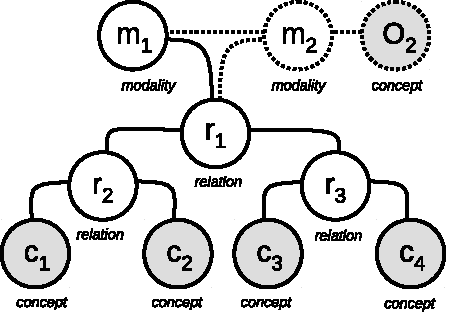
\includegraphics[scale=1]{microstructure.pdf}
      \end{center}
      \caption{Claim microstructure (2nd-order).}
  \label{fig:structures_flowchart}
\end{figure}

Microstructures are structures expressing relations between the domain-specific
concepts, reflecting beliefs, value judgements, or desired policies of the claim
author. Their purpose is to capture the gist of the claim. 
They stemmed from as many claims could be expressed as a \emph{relation}
between \emph{concepts} using a certain \emph{modality}. 
Figure~\ref{fig:structures_flowchart} shows a claim microstructure bringing three elements 
together. 

\paragraph{Relations. }  Many claims can be represented as expressing a
relation between two concepts. For example, on the topic of ``Gay Rights'', 
the relations may be `\texttt{promotes(gay marriage, depopulation)}' and 
`\texttt{purpose(love, procreation)}'. 
There are also comparably fewer claims that can be expressed via
higher-order relations , e.g. `\texttt{entails(constitution, allow(state, gay marriage))}. 
Each relation can be negated, e.g. $\neg$\texttt{promotes(gay marriage,
depopulation)} expresses that gay marriage does not cause depopulation. 
Relations are domain independent. 

\paragraph{Concepts. }
The relations are established between concepts, expressed by noun phrases. 
For ease of access, they can be arranged into a small, domain specific taxonomy of concepts. 
For instance ``gay marriage'', ``heterosexual marriage'' and ``religious marriage''
all belong under the concept of ``marrriage''. 
The taxonomic relations could also be useful for later computational processing. 
Concepts are domain dependent and need to defined for each topic anew

\paragraph{Modalities. }
We observe that claims are expressed under different modalities. 
They can be roughly categorized into \textit{beliefs, value judgements, and policies}. 
We formalize this via unary relations `believes', `approves', `disapproves',
and `desires' corresponding 
to beliefs (factual, religous, and opinion-based), positive value judgements, negative value 
judgements, and desired policy (desired state of affairs) respectively. 
The three modalities act as a wrapper on the propositional content of the claim, 
effectively modulating what is being claimed. 
For instance, `\texttt{believes(purpose(love, procreation))}' expresses the belief 
that love serves procreation, while \texttt{desires(}$\neg$\texttt{allow(state, gay marriage))}'
expresses the wish for the state not to allow gay marriages. 
Finally, in a number of claims the claim is expressed with a reference to a second
opinion holder (e.g. the Bible, the state). 
To tackle this, we add an additional modality layer with the opinion holder as
an additional modifier. 
For instance `\texttt{believes(believes[state](promotes(marriage, advancement)))}' corresponds
to the belief that the state believes gay marriages lead to an advancement. 
By convention, the opinion holder of the first modality is always the author of the post. 

\begin{table}
{\footnotesize
\begin{tabular}{lp{0.80\columnwidth}}
\toprule
\textbf{Relation} & \textbf{Definition} \\
\midrule
\texttt{promotes(A, B)} & Promoting agent A promotes, fosters, leads, increases likelihood, boosts B.  \\
\texttt{suppress(A, B)} & Suppressing agent A suppresses, decreases likelihood, puts down, vanquishes B \\
\midrule
\texttt{allow(A, B)} & Principle A allows, approves, licenses state of affairs B \\
\midrule
\texttt{entails(A, B)} & State of affairs A, necessarily, per definition or causally, makes B true. \\
\texttt{contradicts(A, B)} & State of affairs A, necessarily, per definition or causally, makes B false. \\
\midrule
\texttt{purpose(A, B)} & The purpose of A is B. \\
\midrule
\texttt{equal(A, B)} & State of affairs A is equal to state of affairs B. \\
\midrule
\texttt{has(A, B)} & A has the properties affected by the existence of B.  \\
\bottomrule
\end{tabular}}
\caption{Relation types in claim microstructures.}
\label{tab:microstructures_relations}
\end{table}

\noindent - $\mathcal{R}, \mathcal{C}$, and $\mathcal{M}$ denote the set of relations, concepts and
modalities, respectively \\
- we define a claim microstructure as a quadruple 
$$
(m_1, m_2, o_2, r)
$$ 
where $m_1 \in \mathcal{M}$, and (optionally) $m_2 \in \mathcal{M} \cup \{\epsilon\}$,
$o_2 \in \mathcal{C} \cup \{\epsilon\}$ is the optional second opinion holder, and 
$r = (t, c_1, c_2) \in \mathcal{R}$ is the (possibly higher order) relation 
between two concepts or relations $c_1, c_2 \in \mathcal{C} \cup \mathcal{R}$, 
conveyed by the relation type $t$. \\
- table~\ref{tab:microstructures_relations} lists all possible relation types \\

\section{Ontology}

- here we talk about an alternative approach to structuring claims \\


\begin{figure}
	\centering
\begin{tikzpicture}
\path [mindmap, grow cyclic, level 1/.append style={sibling angle=360/13},
concept color=orange!40,
]
node [concept] {domain topic}[clockwise from=0]
	child { node[concept] {religion}}
	child { node [concept]{plant}}
	child { node[concept] {war}}
	child { node[concept] {organization}}
	child { node[concept] {human being}}
	child { node[concept]  {human rights}}
  child {  node[concept] {plant}}
  child {  node[concept] {status behavior}}
  child {  node[concept] {economic cost}}
  child {  node[concept] {drug}}
  child {  node[concept] {crime}}
  child {  node[concept] {science}}
  child {  node[concept] {disease}};
  child {  node[concept] {society effect}};
	
\end{tikzpicture}
\caption{Marijuana legalization domain ontology classes}
\label{fig:marijuana_domain_ontology}
\end{figure}

\begin{figure}
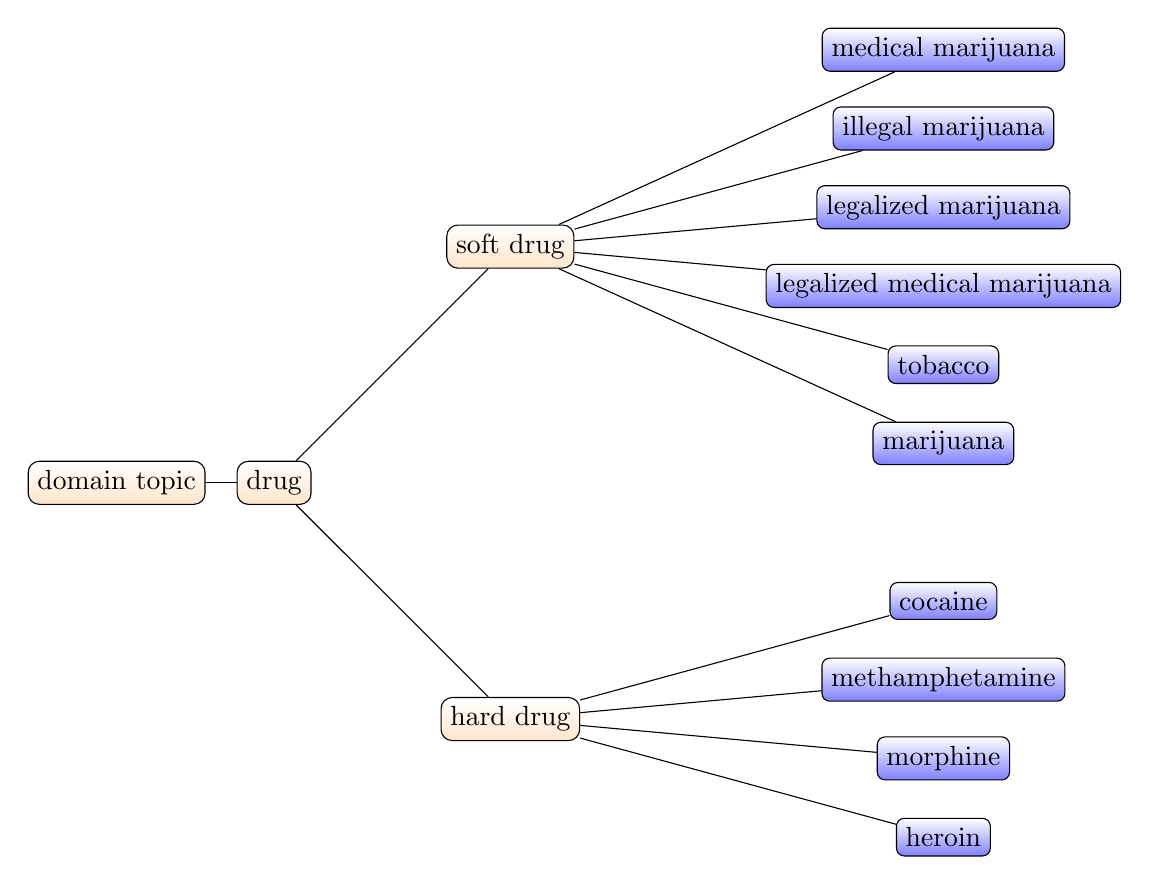
\begin{tikzpicture}
[grow'=right,
level 1/.style={sibling distance=1.5cm, level distance=2cm},
level 2/.style={sibling distance=1.5cm, level distance=3cm, },
level 3/.style={
sibling distance=1cm, level distance=5.5cm},
concept/.style=
{shape=rectangle, rounded corners,
draw, align=center,
top color=white, bottom color=orange!20},
individual/.style={rectangle, rounded corners=1mm, draw, top color=white, bottom color=blue!50,
text centered}
	]
	\node (root) [concept] {domain topic}
	child  { node [concept] {drug}
	child  { node [concept] {soft drug} 
	child { node [individual] {medical marijuana}}
	child { node [individual] {illegal marijuana}}
	child { node [individual] {legalized marijuana}}
	child { node [individual] {legalized  medical marijuana}}
	child { node [individual] {tobacco}}
	child { node [individual] {marijuana}}
    }
    child [missing]
    child [missing]
    child [missing]
    child {node  [concept]{hard drug}
	child {node [individual] {cocaine}}
	child {node [individual] {methamphetamine}}
	child {node [individual] {morphine}}
	child {node [individual] {heroin}}
    }
};
	
\end{tikzpicture}
\caption{Marijuana legalization domain ontology drug individuals. 
	Classes/entities and orange and individuals are blue. }
	\label{fig:drug_domain_individuals}
\end{figure}

\begin{figure}
\begin{tikzpicture}
\end{tikzpicture}
\end{figure}

\begin{figure}
\footnotesize
	\begin{tikzpicture}[
lefttext/.style={rectangle, fill=white,
text width=7cm, text ragged, minimum height=0.5cm},
centertext/.style={rectangle, fill=white,
text width=1.8cm, text ragged, minimum height=0.8cm, align=center},
pro/.style={nodes={fill=green!30}},  
]
\node[matrix of nodes] (mymat) {
	\node [lefttext] (mymat-1-1) {1: There are side effects to smoking marijuana}; &
		\node[centertext] (topleft) {}; &
		\node[centertext] (grid-1-2){}; & 
		\node[centertext] (half-1) {}; &
		\node[centertext] (first) {}; &
		\node[centertext] (grid-1-5){}; & 
		\\[0.5cm]
\node [lefttext] (mymat-2-1) {1: There are side effects to smoking marijuana}; &
		\node[centertext] (grid-2-1){}; &
		\node[centertext] (grid-2-2){}; & 
		\node[centertext] (half-2) {}; &
		\node[centertext] (grid-2-4){}; &
		\node[centertext] (grid-2-5) {}; & 
		\\
		\node [lefttext] (mymat-3-1) {2: Marijuana is not a drug }; &
		\node[centertext] (grid-3-1){}; &
		\node[centertext] (grid-3-2){}; & 
		\node[centertext] (half-3) {}; &
		\node[centertext] (grid-3-4){}; &
		\node[centertext] (grid-3-5){}; & 
		\\[0.5cm]
		\node [lefttext] (mymat-4-1) {1: There are side effects to smoking marijuana}; &
		\node[centertext] (grid-4-1){}; &
		\node[centertext] (grid-4-2){}; & 
		\node[centertext] (half-4) {}; &
		\node[centertext] (grid-4-4){}; &
		\node[centertext] (grid-4-5){}; & 
		\\
		\node [lefttext] (mymat-5-1) {2: Marijuana is not a drug}; &
		\node[centertext] (third) {}; &
		\node[centertext] (grid-5-2) {}; & 
		\node[centertext] (half-5) {}; &
		\node[centertext] (grid-5-4) {}; &
		\node[centertext] (grid-5-5) {}; & 
		\\
		\node[lefttext] (mymat-6-1) {3: Marijuana should be legalized}; &
		\node[centertext] (bottomleft) {} ; &
		\node[centertext] (grid-6-2){}; & 
		\node[centertext] (half-6) {}; &
		\node[centertext] (grid-6-4) {}; &
		\node[centertext] (bottomright) {}; & 
		\\
		&
		\node [centertext] {Definitely Pro};  & 
		\node [centertext] {Probably Pro}; & 
		\node [centertext] {Neutral }; & 
		\node [centertext] (kre) {Probably Con}; & 
		\node [centertext] (bla) {Definitely Con}; \\
};

\draw[fill=green!30, draw=none] (topleft.north west)
rectangle ($(half-6.south west)!0.5!(half-6.south east)$);

\draw[fill=red!30, draw=none] ($(half-1.north west)!0.5!(half-1.north east)$)
rectangle (bottomright.south east);

% circles
% \draw ($(first.base) + (-0.2cm, 0.1cm)$) circle (0.2cm) node {\tiny{x}};
% \draw ($(half-3.base) +(-0.0005cm, 0.4cm) $) circle (0.2cm) node {\tiny{x}};
% \draw ($(third.base) + (0, 0)$) circle (0.2cm) node {\tiny{x}};

% x-marks the spot
%lower
\draw[thick] ($(bottomleft.south west) + (0.1cm, 0.1cm)$) -- 
($(grid-4-1.north east)$);
\draw[thick] ($(bottomleft.south east) + (0, 0.1cm)$) -- 
($(grid-4-1.north west) + (0.1cm, 0)$);

%middle
\draw[thick] (half-3.south west) -- 
(half-2.north east);
\draw[thick] (half-2.north west) -- 
(half-3.south east);

%upper
\draw[thick] ($(first.south west) + (0.3cm, -0.1cm)$) --
($(first.north east) + (-0.3cm, -0.1cm)$ );
\draw[thick] ($(first.north west) + (0.3cm, -0.1cm)$) -- 
($(first.south east) + (-0.3cm, -0.1cm)$);

% horizontal lines
% lower
\node[fit=(bla) (kre), inner sep=0pt] (R5) {};
\draw [thick] ($(R5.north -| mymat.west) + (0, 0.1cm)$)  -- ($(R5.north -| mymat.east) + (0, 0.1cm)$);

%upper
\node[fit=(mymat-1-1), inner sep=0pt] (R4) {};
\draw [thick] ($(R4.north -| mymat.west) + (0, 0.05cm)$)  -- 
($(R4.north -| mymat.east) + (0, 0.05cm)$);
 
%mid-1
\node[fit=(mymat-2-1), inner sep=0pt] (R2) {};
\draw ($(R2.north -| mymat.west) + (0.2cm, 0.4cm)$) -- ($(R2.north -| mymat.east) + (-0.2cm,0.4cm)$);

%mid-2
\node[fit=(mymat-4-1), inner sep=0pt] (R3) {};
\draw ($(R3.north -| mymat.west) + (0.2cm, 0.4cm)$) -- ($(R3.north -| mymat.east) + (-0.2cm,0.4cm)$);

% vertical line
\draw ($(topleft.north west)$) -- ($(bottomleft.south west)$);

\end{tikzpicture}
\caption{Shifts pro con. The stance changes as more claims are uncovered. In the first row, 
a single claim is known, based on which the \textbf{con} stance is inferred.
The stance shifts as the second and third claim are uncovered towards neutral and 
\textbf{pro} stance, respectively. 
}
\label{fig:pro_con_shift}
\end{figure}

\begin{figure}
	\centering
	\footnotesize
	\begin{tikzpicture}[
concept/.style={shape=rectangle, rounded corners,
draw, align=center,
top color=white, bottom color=orange!20},
node distance=5cm,
]
\node [concept] (human) {human being};
\node [concept, below right of=human] (domain) {domain topic};
\node [concept, above left of=human] (disease) {disease};
\node [concept, below left of=human] (status) {status behavior};
\node [concept, above right of=human] (drug) {drug};

\draw[densely dashed, color=olive] (human) -- (domain);
\draw[densely dashed, color=olive] (disease) .. controls ($(human) + (-1.3cm, -1.3cm)$) .. (domain); 
\draw[densely dashed, color=olive] (status) -- (domain); 
\draw[densely dashed, color=olive] (drug) -- (domain); 
\draw[densely dashed, color=olive] (human) -- (domain); 

		\draw [->] (human.north) .. controls ($(human.north) + (0cm,
		3cm)$) ..  (drug) node [sloped, above, near end] {buys drugs}; 
		\draw [->] (human.north) .. controls ($(human) + (3.5cm, 1cm)$)
		..  (drug) node [sloped, above, near start] {consumes drugs}; 
		\draw [->] (human) -- (status) node [below, midway, sloped] {has behavior}; 
		\draw [->] (human) -- (disease) node [below, midway, sloped] {has disease}; 
\end{tikzpicture}
	\caption{Dashed lines indicate subclass, full lines indicate object property relations. 
	The triple (\texttt{human\_being}, \texttt{buys\_drugs}, \texttt{drug}) represents an 
	individual that belongs to the
	\texttt{human\_being} class, which posses the property \texttt{buys\_drugs} with 
	object \texttt{drug}.} 
	\label{fig:main-classes}
\end{figure}
